\documentclass[11pt]{article}
\usepackage[utf8]{inputenc}

% add LaTeX packages to use here
\usepackage{amsmath}
\usepackage{amssymb}
\usepackage{amsfonts}
\usepackage{amsthm}
\usepackage{fancyhdr}
\usepackage{lastpage}
\usepackage{enumitem}
\usepackage{framed}
\usepackage[most]{tcolorbox}
\usepackage{geometry}
\usepackage{graphicx}

 % set dimensions for page layout
\geometry
{
 left=5em,
 right=5em,
 bottom=5em,
 top=6em,
 headheight=110pt,
 showframe=false
}

\setlist[itemize]{leftmargin=*} % prevents indenting of itemize

% abbreviations for some common math symbols
\newcommand{\Rset}{\hbox{$\mathbb R$}}
\newcommand{\Nset}{\hbox{$\mathbb N$}}
\newcommand{\Pset}{\hbox{$\mathbb{N}^{+}$}}
\newcommand{\Zset}{\hbox{$\mathbb N$}}
\newcommand{\Qset}{\hbox{$\mathbb Q$}}

% theorem style
\newtheoremstyle{thmstyle}% name of the style to be used
  {0pt}% measure of space to leave above the theorem. E.g.: 3pt
  {0pt}% measure of space to leave below the theorem. E.g.: 3pt
  {}% name of font to use in the body of the theorem
  {}% measure of space to indent
  {\bfseries}% name of head font
  {.}% punctuation between head and body
  { }% space after theorem head; " " = normal inter-word space
  {}% Manually specify head

% theorem environment instance
\theoremstyle{thmstyle}
\newtheorem{theorem}{Theorem}

% shaded and framed solution environment
\makeatletter
\newenvironment{shadedSolutionBox}
  {\setlength{\OuterFrameSep}{0in}%
  \definecolor{shadecolor}{gray}{.8}% shading of shaded solution box
  \bigskip%
  \@nameuse{shaded*}\par\noindent\ignorespaces \textit{Solution}.}
  {\hspace{\stretch{1}}\rule{1.5ex}{1.5ex}% adds filled box
  \@nameuse{endshaded*}%
  \bigskip}
\makeatother

% shaded and framed theorem environment
\makeatletter
\newenvironment{thm}
  {\setlength{\OuterFrameSep}{0in}%
  \definecolor{shadecolor}{gray}{1}% shading of shaded Theorem box
  \@nameuse{snugshade*}\par\noindent\ignorespaces%
   \@nameuse{theorem}}
  {\hspace{\stretch{1}}\scalebox{1.5}{\hbox{$\triangleleft$}}% adds triangle shape
  \@nameuse{endtheorem}%
  \@nameuse{endsnugshade*}%
  }
\makeatother

% header and footer elements of every page except the first.
\pagestyle{fancy}
\fancyfoot[L]{\textsc{CISC {\small\selectfont 3230}} }
\fancyhead[R]{{\small\selectfont\textsc{\studentLastName}}}
\fancyfoot[C]{{\small\selectfont\assignmentName}}
\fancyfoot[R]{{\small\selectfont\thepage\ of \pageref{LastPage}}}
\renewcommand{\headrulewidth}{0.8pt}
\renewcommand{\footrulewidth}{0.4pt}

% hline with variable thickness
\makeatletter
\def\thickhline{%
  \noalign{\ifnum0=`}\fi\hrule \@height \thickarrayrulewidth \futurelet
   \reserved@a\@xthickhline}
\def\@xthickhline{\ifx\reserved@a\thickhline
               \vskip\doublerulesep
               \vskip-\thickarrayrulewidth
             \fi
      \ifnum0=`{\fi}}
\makeatother

% length instance for \thickhline
\newlength{\thickarrayrulewidth}
\setlength{\thickarrayrulewidth}{.8pt}

% header and footer for first page
\fancypagestyle{firstpage}
{
\fancyhf{}
\renewcommand{\footrulewidth}{0.4pt}
\renewcommand{\headrulewidth}{0pt}
\fancyhead[C]{%
\begin{tabular*}{\textwidth}{@{\extracolsep{\fill}}@{}l @{} c @{} r @{} }
{\small\selectfont\courseName}&{\normalsize\selectfont\assignmentName}&{\small\selectfont\studentFirstName\ \studentLastName}\\
\thickhline
&&{\scriptsize\selectfont\collaboratorNames}
\end{tabular*}%
}
\fancyfoot[R]{{\small\selectfont\thepage\ of \pageref{LastPage}}}
\fancyfoot[L]{{\footnotesize\selectfont\pdfcreationdate}}
}

\newcommand{\courseName}{Theoretical Computer Science} % course name

% your first name, your last name, and the assignment name
\newcommand{\studentLastName}{Nikabadze} % your last name
\newcommand{\studentFirstName}{Luka} % your first name (and middle name, if applicable)
\newcommand{\assignmentName}{Assignment 2 CISC3230} % the assignment name
\newcommand{\collaboratorNames}{[First Name Initial]. Last Name} % if you worked with anyone to complete any part of the assignment, include the initial of the first name (and middle name, if applicable) and full last name of each of your collaborators, separated by commas (e.g., if you worked with Arthur Paul Pedersen and Sandra Lee, include "A.P. Pedersen, S. Lee")




\begin{document} % marks the beginning of the document

\thispagestyle{firstpage} % institutes page style for first page

\setlength{\abovedisplayskip}{20pt} % space above math in align* environment
\setlength{\belowdisplayskip}{20pt} % space below math in align* environment



% marks the beginning of the document body

\begin{itemize}\setlength{\itemsep}{1em} % \itemsep is the spacing between items in environment




\begin{center}
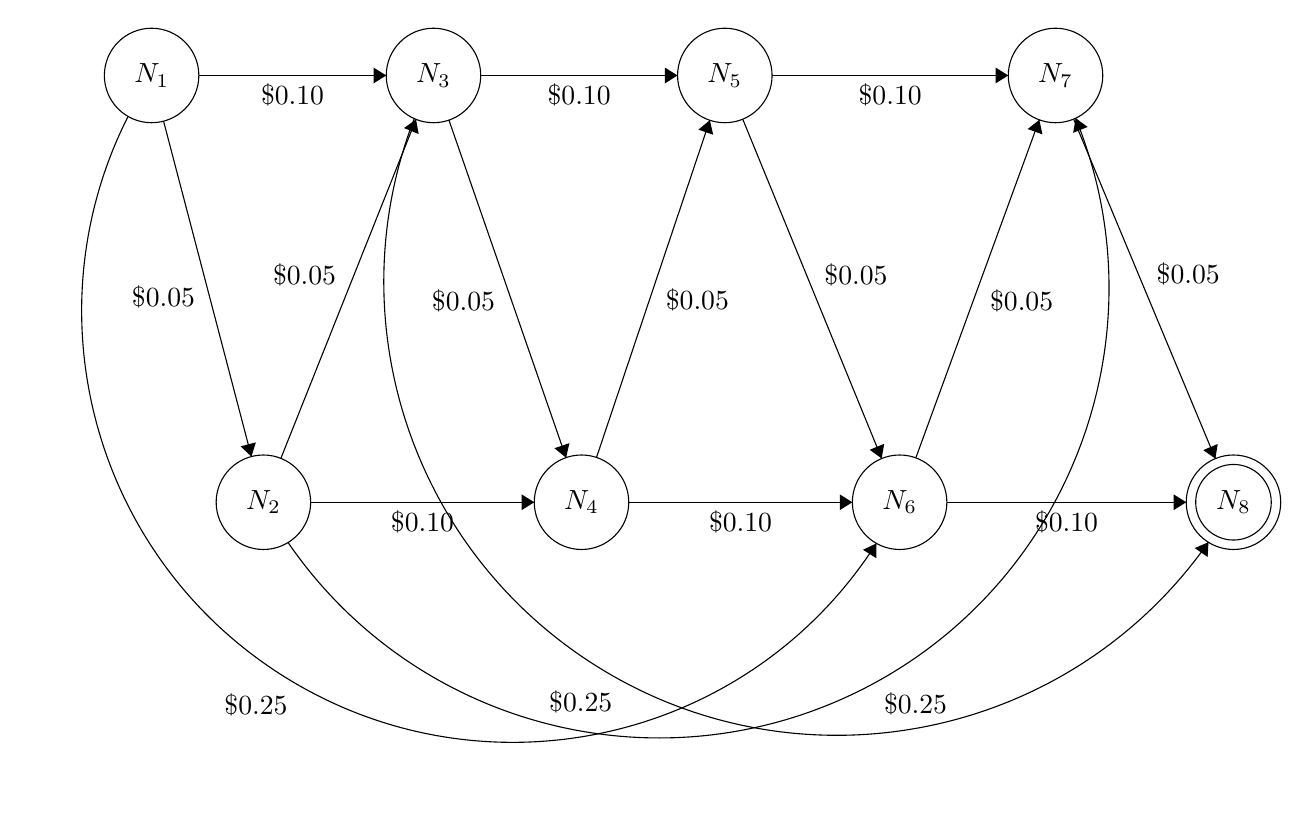
\begin{tikzpicture}[scale=0.2]
\tikzstyle{every node}+=[inner sep=0pt]
\draw [black] (13.2,-39.3) circle (3);
\draw (13.2,-39.3) node {$N_2$};
\draw [black] (24,-12.2) circle (3);
\draw (24,-12.2) node {$N_3$};
\draw [black] (42.5,-12.2) circle (3);
\draw (42.5,-12.2) node {$N_5$};
\draw [black] (63.5,-12.2) circle (3);
\draw (63.5,-12.2) node {$N_7$};
\draw [black] (74.8,-39.3) circle (3);
\draw (74.8,-39.3) node {$N_8$};
\draw [black] (74.8,-39.3) circle (2.4);
\draw [black] (33.4,-39.3) circle (3);
\draw (33.4,-39.3) node {$N_4$};
\draw [black] (53.6,-39.3) circle (3);
\draw (53.6,-39.3) node {$N_6$};
\draw [black] (6.1,-12.2) circle (3);
\draw (6.1,-12.2) node {$N_1$};
\draw [black] (14.31,-36.51) -- (22.89,-14.99);
\fill [black] (22.89,-14.99) -- (22.13,-15.54) -- (23.06,-15.92);
\draw (17.85,-24.87) node [left] {$\$0.05$};
\draw [black] (64.65,-14.97) -- (73.65,-36.53);
\fill [black] (73.65,-36.53) -- (73.8,-35.6) -- (72.88,-35.99);
\draw (69.89,-24.82) node [right] {$\$0.05$};
\draw [black] (27,-12.2) -- (39.5,-12.2);
\fill [black] (39.5,-12.2) -- (38.7,-11.7) -- (38.7,-12.7);
\draw (33.25,-12.7) node [below] {$\$0.10$};
\draw [black] (45.5,-12.2) -- (60.5,-12.2);
\fill [black] (60.5,-12.2) -- (59.7,-11.7) -- (59.7,-12.7);
\draw (53,-12.7) node [below] {$\$0.10$};
\draw [black] (24.98,-15.03) -- (32.42,-36.47);
\fill [black] (32.42,-36.47) -- (32.63,-35.55) -- (31.68,-35.87);
\draw (27.94,-26.49) node [left] {$\$0.05$};
\draw [black] (34.35,-36.46) -- (41.55,-15.04);
\fill [black] (41.55,-15.04) -- (40.82,-15.64) -- (41.76,-15.96);
\draw (38.72,-26.46) node [right] {$\$0.05$};
\draw [black] (16.2,-39.3) -- (30.4,-39.3);
\fill [black] (30.4,-39.3) -- (29.6,-38.8) -- (29.6,-39.8);
\draw (23.3,-39.8) node [below] {$\$0.10$};
\draw [black] (36.4,-39.3) -- (50.6,-39.3);
\fill [black] (50.6,-39.3) -- (49.8,-38.8) -- (49.8,-39.8);
\draw (43.5,-39.8) node [below] {$\$0.10$};
\draw [black] (56.6,-39.3) -- (71.8,-39.3);
\fill [black] (71.8,-39.3) -- (71,-38.8) -- (71,-39.8);
\draw (64.2,-39.8) node [below] {$\$0.10$};
\draw [black] (43.64,-14.98) -- (52.46,-36.52);
\fill [black] (52.46,-36.52) -- (52.62,-35.59) -- (51.7,-35.97);
\draw (48.79,-24.84) node [right] {$\$0.05$};
\draw [black] (54.63,-36.48) -- (62.47,-15.02);
\fill [black] (62.47,-15.02) -- (61.73,-15.6) -- (62.67,-15.94);
\draw (59.31,-26.54) node [right] {$\$0.05$};
\draw [black] (6.86,-15.1) -- (12.44,-36.4);
\fill [black] (12.44,-36.4) -- (12.72,-35.5) -- (11.75,-35.75);
\draw (8.89,-26.24) node [left] {$\$0.05$};
\draw [black] (9.1,-12.2) -- (21,-12.2);
\fill [black] (21,-12.2) -- (20.2,-11.7) -- (20.2,-12.7);
\draw (15.05,-12.7) node [below] {$\$0.10$};
\draw [black] (52.125,-41.911) arc (-32.60072:-206.81107:27.391);
\fill [black] (52.13,-41.91) -- (51.27,-42.32) -- (52.12,-42.85);
\draw (12.73,-51.45) node [below] {$\$0.25$};
\draw [black] (64.776,-14.914) arc (22.17942:-145.55074:28.568);
\fill [black] (64.78,-14.91) -- (64.62,-15.84) -- (65.54,-15.47);
\draw (54.61,-51.36) node [below] {$\$0.25$};
\draw [black] (73.208,-41.841) arc (-35.05291:-201.10377:28.793);
\fill [black] (73.21,-41.84) -- (72.34,-42.21) -- (73.16,-42.78);
\draw (33.35,-51.22) node [below] {$\$0.25$};
\end{tikzpicture}
\end{center}

{\textbf{As you can see above there are total 8 states. $N_1$ is first node and it goes till 8.  Basically each next node counts as $0.05$ cents as result we can see that after adding each state which also adds $0.05$ cent gives us in total $0.35$ which is final state $N_8$. In case of $0.10$ it is added every other $2nd $ node for example if first coin is $0.10$ cent it goes on $N_3$ state then if $2nd $ coin is $0.05$ cent it will go on $N_4$ state, but if  $2nd $ coin is  $ 0.10$ cent as well it will go $N_5 $ node and so on until it goes until $0.35$ cent. Then as we can see $0.25$ can only be $1st$ $2nd $ or $3rd$ coin. Because if it is $4th$ then it will be more than $0.35 $ cent.}}

\begin{align*}
\end{align*}
\end{itemize}


\end{document}